\begin{savequote}[75mm]

... As for me, nothing in the universe can be the same if somewhere, no one knows where, a sheep we never saw has or has not eaten a rose....
Look up at the sky. Ask yourself, ``Has the sheep eaten the flower or not?" And you'll see how everything changes....
And no grown-up will ever understand how such a thing could be so important!
\qauthor{Antoine de Saint-Exup{\^e}ry (The Little Prince)}
\end{savequote}


\chapter{Introduction}
\label{introduction}

\section{A Brief History of Galaxy Evolution}

\subsection{The Discovery of Galaxies}
One of the momentous shifts in scientific thinking was the realization that our Sun might be one of many stars in the Universe. From this sprung the idea that perhaps the gravitationally bound system of stars, stellar remnants, gas and dust that the Sun is a part of is one of many such structures known as galaxies. The bright band of stars and dust that we observe in the night sky, which we now know as our own galaxy, the Milky Way, has been a puzzling topic since ancient times. The Greek philosopher Democritus is known to have speculated that this might be a band of distant stars but the thought was left by the wayside with the advent of Aristotelian physics. The astronomers of medieval Islam, such as Alhazen, al-Biruni and Ibn-Bajjah, centuries later, also hypothesized that the Milky Way was made of many stars such as our own Sun. However, observational proof for this came only in the 17th century when the Italian astronomer, Galileo Galelei pointed his telescope at this band and confirmed that the Milky Way was indeed made up of a huge number of faint stars.\\

Since the debate on a geocentric versus heliocentric Universe was still ongoing, Galileo's observations weren't given credence until more than century later, during which time, the development of Keplerian orbital mechanics and Newtonian Theory of Gravitation had resulted in a successful explanation of the Solar System and its dynamics. The idea that the galaxy might be a rotating configuration of a huge number of stars held together by gravitational forces that contained smaller gravitationally bound configurations such as our Solar System was first theorized by the English astronomer, Thomas Wright, in 1750. On the heels of his observation that the faint (then so-called) ``nebulae" observed might be distant galaxies that came out of ``external creations", philosopher Immannuel Kant hypothesized the existence of many such ``island Universes" and speculated that these could potentially form and evolve independently from our own, thus laying the underpinnings of the study of galaxy formation and evolution.\\

\subsection{Early Studies of Galaxies}

William Herschel, in the 1780s, surveyed the stars in the Milky Way in multiple directions and discovered that the density of stars was greater on one side than the other. One of the earliest catalogues of galaxy-like objects was developed by Charles Messier, also towards the end of the 18th century, following which William Herschel assembled a catalog of 5000 nebulae. In the 19th century, with advances in optics and instrumentation, the first telescope to distinguish between elliptical and spiral galaxies was built by Lord Rosse. Additionally, this telescope could resolve point sources within the nebulae, thus confirming that galaxies were indeed ``island universes" as Wright and Kant had surmised.\\

In early 20th century, astronomers were beginning to get interested in the chemical composition of these nebulae and started recording their spectra. With the advent of Einstein's Special Theory of Relativity, one could calculate the radial velocity of a ``nebula" based on how its spectrum is Doppler-shifted. And so it happened that the American astronomer, Vesto Slipher, became the first person to measure galactic redshifts in 1912. While studying the chemical composition of bright spiral nebulae, he noticed that they were all highly Doppler-shifted, with estimated radial velocities that were much higher than the velocities of stars in the Milky Way. He also noticed that there were more ``red-shifted" (i.e. moving away from us) nebulae than ``blue-shifted" ones, an observation that would later propel Edwin Hubble to propose that the Universe was expanding.\\

In the 1920s, a series of observations made by Edwin Hubble, Ernst Opik, etc., confirmed that Andromeda was not a part of the Milky Way and was a galaxy is its own right, thus effectively settling the ``Great Debate" of the times and confirming that our galaxy was just one of many galaxies in the Universe. Georges Lema{\'i}tre, a Belgian physicist, predicted, on theoretical grounds rooted in Einstein's General Theory of Relativity, that the redshifts of galaxies should increase with distance. In 1929, Edwin Hubble looked at the distances and velocities of 46 galaxies and observed the same \citep{1929PNAS...15..168H}: that their radial velocities increased with distance from us, thus theorizing what we know today as Hubble's Law (or alternately, the Hubble-Lema{\'i}tre Law). Edwin Hubble further analyzed the morphologies of these galaxies and came up with the Hubble Sequence, a classification of galaxy morphology (Fig. \ref{fig:hubble_classification}). The Swiss astrophysicist, Fritz Zwicky, in 1933, while studying galaxy clusters, noticed that the orbits of the galaxies were not accounted for by the mass of its luminous components, leading him to believe that there must be some ``missing" mass \citep{1937ApJ....86..217Z} that does not interact electromagnetically, thus remaining unseen and termed it \emph{dunkle Materie}, i.e.,``dark matter".\\

Thus with the emergence of new theories of spacetime, an expanding Universe that (as it was termed later) began with a ``big bang", the existence of matter that doesn't interact electromagnetically, the study of galaxies in the 1930s set in motion a paradigm shift for astronomy and cosmology. The new questions were: How were the earliest galaxies formed? What would explain the diversity in morphologies seen in galaxies today? Is the Universe set to expand indefinitely? What drives the expansion of the Universe? What is dark matter? If the Universe's origins were homogeneous, how do we explain the heterogenous nature of the populations of galaxies seen?\\

\subsection{Galaxy Evolution and Cosmology}

The explorations in the latter half of the 20th century confirmed a few of the hypotheses discussed above, along with answering a few of those questions. In the 1960s and 1970s, Vera Rubin, Kent Ford, and Ken Freeman analyzed rotation curves of spiral galaxies and provided strong evidence for the existence of dark matter \citep{freeman_disks_1970-1}. Rubin inferred that most galaxies contain around six times as much dark matter as visible mass \citep{rubin_rotational_1980}, thus placing new constraints on galaxy formation and evolution in the Universe.\\

The two predominant theories of the origin of the Universe were: the ``Big Bang Theory", originally proposed by Georges Lema{\'i}tre, and the ``Steady State Theory" (essentially an unchanging Universe whose density remains the same in spite of expansion due to continuous creation of matter) proposed by Fred Hoyle. However, with theories of Big Bang Nucleosynthesis (the $\alpha\beta\gamma$ paper; \citealt{alpher_origin_1948}) that successfully explained how the elements of the of the Universe came to be formed after the Big Bang and radio source counts which were also correctly accounted for by the Big Bang Theory swung cosmologists to favor this over the Steady State Theory. The final nail in the coffin was the successful detection of the Cosmic Microwave Background (CMB), predicted by the Big Bang Theory \citep{1965ApJ...142..419P}. According to the Big Bang Theory, the early Universe cools from a very hot state and remains an ionized plasma for the first few hundred thousand years (until redshift $z\sim 1100$). The emission from this era should be a Planck spectrum of the plasma at about the time that hydrogen recombines, redshifted due to the universe's expansion since then. This model predicts a spectrum peaking at near microwave wavelengths today, and the CMB is indeed detectable as a very low energy radiation with a blackbody temperature of \~ 3K.\\

The discovery of dark matter coupled with the confirmation of the Big Bang Theory necessitated a theory of dark matter that would successfully explain the observable Universe. In the 1980s, competing theories of hot and cold dark matter \citep{1985ApJ...292..371D} were proposed. Eventually the cold dark matter theories won out as their prediction of the anisotropies in the CMB \citep{peebles_large-scale_1982} were successfully verified by the Cosmic Background Explorer (COBE) probe \citep{smoot92a} in combination with other data sets.\\

Before the turn of the century, the remarkable discovery of the accelerating universe \citep{Riess:1998cb} resulted in the resurrection of Einstein's cosmological constant and effectively confirmed $\Lambda$CDM as the clear winner among the cold dark matter models. The Big Bang Theory, together with the $\Lambda$CDM model, forms much of the basis of modern cosmology and the foundations for theories of galaxy formation and evolution.\\

\section{Galaxy Formation and Evolution}

\subsection{Structure Formation in the Universe}
The current model of cosmology suggests that there was a single event, the so-called ``Big Bang" which resulted in the appearance of expanding space-time containing radiation, followed by an exponential expansion of space known as cosmic inflation \citep{PhysRevD.23.347} which established the initial properties of the Universe as being homogeneous, isotropic and flat. Tiny perturbations in this early Universe are responsible for structure formation. Cosmic inflation also explains the fact that these tiny quantum fluctuations grow into slight ripples of over-density and under-density thus seeding the early stages of structure formation in the Universe.\\

From a predominantly radiation-dominated Universe, with expansion, the density of radiation drops steeply leading to a the matter-radiation equality at ~ 50,000 years after the Big Bang. Since dark matter only interacts gravitationally, the dark matter ripples from the fluctuations form compact structures more freely as they are not opposed by other forces such as radiation pressure.\\

About 380,000 years after the Big Bang, the expansion of the Universe resulted in a lowering of density as well as a cooling down of its temperature to a point where protons and electrons in this plasma soup start combining to form the neutral hydrogen. Electrons decouple from the photons (these decoupled photons are what we detect as the CMB today) and the baryonic matter is now free to collapse under gravity creating local over-densities.\\

As fluctuations continue to grow, ever larger scales enter the non-linear regime of structure formation where dense concentrations of matter (dark and baryonic alike) get progressively denser. 
Dark matter begins to collapse into structures known as halos, and baryons fall with the dark matter into these halos. These structures arrange themselves into gravitationally stable configurations, a process known as virialization.
The result of this process gives rise to a Universe that resembles a web (the cosmic web) with sheets and filaments of dark matter, creating a skeletal backbone in which star formation and galaxy formation eventually occur.

Within the dark matter halos baryonic matter can, when it becomes dense enough, additionally lose energy by radiation and can sink further into regions of high over-density. 
The stars and galaxies have their origins in these structures and are the resulting of the cooling of baryons deep in the potential wells of dark matter halos.

While a short summary of how galaxies form would be that the collapse of baryonic matter within dark matter halos results in disk-like structures that then collapse on small scales to form stars, the mechanisms by which this happens is still a topic of debate among astrophysicists. While a top-down scenario, wherein disk galaxies were formed from the collapse of a single large cloud of gas \citep{1962ApJ...136..748E}, captures some stages of galaxy formation well, in fact both theory and observations suggest that galaxies grow hierarchically --- small galaxies form and merge into larger ones --- which complexifies the picture. Meanwhile, the overall efficiency with which baryons form stars depends strongly on the halo mass (e.g. \citealt{behroozi_comprehensive_2010}), peaking at masses similar to that of the Milky Way. As \citet{somerville15a} describe, this dependence probably arises from processes that suppress star formation at lower masses (perhaps due to supernova feedback) and at higher masses (perhaps due to feedback from accreting supermassive black holes).

% Prior to the establishment of $\Lambda$CDM as the dominant cosmological model, the popular theory of galaxy formation was the top-down scenario \citep{1978ApJ...225..357S} which proposed that disk galaxies were formed from the collapse of a single large cloud of gas \citep{1962ApJ...136..748E} into disks that pushed the dark matter out into halos. The cooling of this rotating disk results in gravitational instabilities that causes smaller clumps of clouds to collapse to form stars. However, the natural prediction of $\Lambda$CDM is a bottom-up scenario wherein the dark matter halos form and 
% (\citet{0004-637X-490-2-493, 2015PNAS..11212249W}) before the formation of the galactic disks.\\

Since we are limited in our observations by the fact that we cannot observe galaxies in a time-resolved fashion (the time scales are too long), theories regarding galaxy formation rely computational simulations that evolve the initial conditions to the present day. We can compare the galaxies at each epoch to the populations observed at different redshift, assuming large scale homogeneity. As \citet{somerville15a} describe, these simulations incorporate the physics of $\Lambda$CDM, magnetohydrodynamics, and gravitation. Additionally, these models need to account for a variety of processes on subresolution scales that involve star formation, stellar and AGN feedback, and gas cooling to be able to correctly predict the observed Universe.\\

\begin{figure}
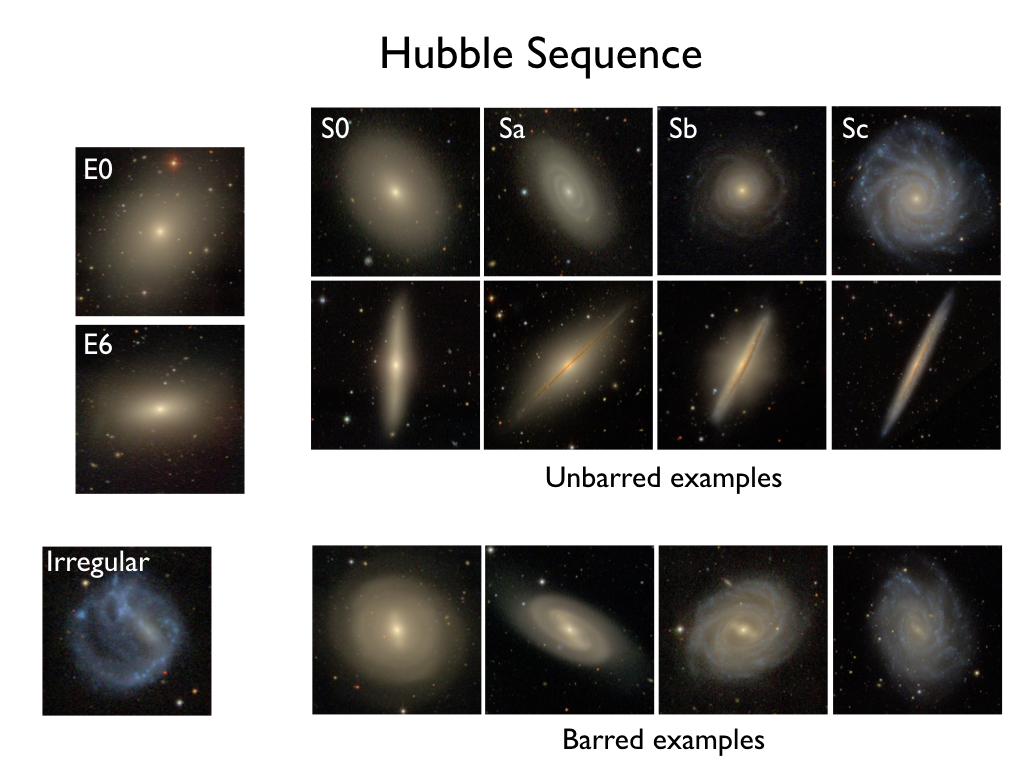
\includegraphics[width=\textwidth]{figures/hubble.jpeg}
\caption[ The Hubble Sequence: A classification scheme for galaxy morphologies (Photo credit: ?)]
{The Hubble Sequence: A classification scheme for galaxy morphologies (Photo credit: ?)
\label{fig:hubble_classification}}
\end{figure}

Thus, there are still many questions to be answered including and not limited to: how and where the baryons collapse, how galactic disks stabilize, the drivers and mechanisms of galactic feedback and what ultimately causes the relative frequency of different galaxy types in the observable Universe. There are thus many holes in this narrative of galaxy formation and evolution and astronomers are working to bridge this gap in two main ways: from the observational side, this involves accurate measurements of galaxy properties across cosmic time and from the (theoretical) side of computational astrophysics, this involves fine-tuning the sub-grid models of galaxy formation and evolution simulations so as to be able to reproduce the estimated from the properties. These both take from and in turn inform the parameters in the $\Lambda$CDM model of the Universe that cosmologists are engaged in refining.\\

\subsection{Galaxy Properties in the Observable Universe}

The commonly used classification scheme for galaxies based on their most obvious attribute, the morphologies of their luminous components, was invented by Edwin Hubble in 1926. The classification scheme is based on the relative sizes and of the bulges and disks in galaxies and broadly encompasses four types of morphologies: elliptical, lenticular, spiral and irregular (Fig. \ref{fig:hubble_classification}). Galaxy morphologies are strongly correlated with their other physical properties such as luminosity, age, chemical composition, star formation histories and kinematics (\citealt{roberts94a}). The bulges usually contain older, redder stars and the disks are characterized by mixed stellar populations along with gas and dust. The disks may also contain spiral arms which usually contain pockets of star formation activity. Elliptical galaxies have almost no disk. Lenticulars are smooth like ellipticals but contain a puffy, thick disk that when observed obliquely has a distinct oval-like appearance (lentil-shaped!). Spirals can have a bulge but are characterized by their thin disk, often with spiral arms. Irregulars are akin to spirals but as their name suggests, appear less organized in their light distribution. Early ideas about galaxy evolution suggested that galaxies formed as ellipticals or lenticulars (referred to as `early-type' galaxies) and later evolved into spirals or irregulars (referred to as `late-type' galaxies) and while there are strong correlations between galactic structure and their star formation rates, it is now known that this is in general untrue.\\

The total amount of light we observe emanating from a galaxy is the
second obvious trait that lends itself to comparison. This can be
quantified as ``luminosity,'' the amount of energy emitted by a star
per unit time, often measured in units of the solar luminosity
$L_{\odot}$, and usually measured in a particular wavelength
bandpass. Optical or near-infrared luminosity can serve as a
reasonable (but not exact) proxy for stellar mass; ultraviolet
luminosity can serve as a reasonable (but not exact) proxy for
current star formation activity. Observations reveal that fainter
galaxies are more frequent per unit volume than galaxies as bright
as our own. Very bright big ellipticals are much rarer than both.
The distribution of galaxy luminosites, per volume and per unit
luminosity, is known as the ``luminosity function''
(\citet{1988MNRAS.232..431E, blanton05a}), which provides key
constraints on galaxy formation and evolution.

The total luminosity of a galaxy in the ultraviolet through near
infrared is generally dominated by stars, and the stellar population
is changing with time as stars evolve off the main sequence and reach
their fates, for example as black holes, neutron stars, or white
dwarfs.  A more stable and sometimes more interesting quantity is the
total mass in stars, the stellar mass. Because the luminosities of
stars varies as $L\propto M^{-\alpha}$, where $\alpha \sim 3$--$5$,
and the more massive stars die rapidly, the total ratio of luminosity
to stellar mass varies over time. Furthermore, because the massive
stars are very hot, the overall color of the stellar population starts
out blue and becomes increasing red. This pattern leads to a
relationship between the galaxy spectrum and the stellar mass to light
ratio, that can be exploited to estimate the stellar mass of a galaxy.

The most basic measure of the spectral energy distribution of galaxies
are its colors.  Colors in astronomy are defined on the basis of the
ratios of observed fluxes in various bandpasses. For instance, $g-r$
is $2.5\log_{10}$ of the ratio of the $r$-band to $g$-band flux, where
$g$ and $r$ are optical bandpasses used in the Sloan Digital Sky
Survey (SDSS); larger $g-r$ indicates a redder galaxy.  Galaxy
populations have a bimodal distribution and can be divided into the
so-called ``red sequence" and ``blue cloud"
(\citet{2001AJ....122.1861S, 2003ApJ...594..186B}). The blue cloud is
dominated by star-forming blue spirals with young stellar populations;
the red sequence has a mixture of varied populations, including some
older or dust-reddened spirals, lenticular galaxies, and ellipticals.
The intermediate colored population, the so-called ``green valley",
must contain (but does not only contain) the population of galaxies
that are in the process of ending their star formation and
transitioning from blue to red. However, a complication to this simple
interpretation of the observations is the presence of dust, which has
the tendency to make galaxies appear redder. We investigate the star
formation of galaxies in the context of optical colors and dust,
further in Chapter \ref{ch:sfrk}.\\

The last significant observable property we introduce here is the
galaxy environment, which is a measure for each galaxy of how many
other galaxies are nearby it relative to the mean galaxy density.
Galaxies exhibit substantial clustering relative to a Poisson
distribution, leading to a large dynamic range in local density For
example, a galaxy like the Milky Way most commonly has not similarly
massive neighbors within 1 Mpc, but massive clusters of galaxies have
100s of Milky Way-sized galaxies within a Mpc. This clustering of
galaxies reveals information about cosmological parameters, like the
initial amplitude of fluctuations and the mean dark matter density.

The environment of galaxies also appears to be correlated with their
formation history, as manifested by their morphology
\citep{dressler_galaxy_1980}, luminosity \citep{2002MNRAS.332..827N},
star formation rates \citep{2002MNRAS.334..673L}, and numerous other
properties. For instance, simplistically, blue galaxies preferentially
exist in isolated environments (or voids) and large red ellipticals
preferentially exist in clusters. Galaxy environments can be measured
in a variety of ways, such as counts in a projected aperture or
distance to nearest neighbor \citep{cooper_measuring_2005}. The
density field length scales at which galaxy environment matters
significantly enough to affect its star formation has been
investigated; it appears that the local environment (within 1--2 Mpc)
is most important, with the larger scale environment being of much less
importance at a fixed local environment
(\citet{kauffmann_environmental_2004, 2006ApJ...645..977B,
  2007ApJ...658..898P}).\\

 
\subsection{Questions in Galaxy Evolution}

The lifecycle of a galaxy can be thought of in terms of the timeline
of the events between the formation of the first stars in the galaxy
began to when there is little to no star formation activity in the
galaxy, i.e. the galaxy is quenched. Many processes determine the
history of star formation and how it may end.  Star formation begins
with the inflow of gas, its formation into galactic disk structures,
its radiatively cooling, the formation of molecular clouds, and the
formation of stars. The stars form in some initial mass distribution
whose form in the Milky Way is constrained observationally, but whose
variation among galaxies is largely unknown. The massive stars in the
stellar mass distribution tend to disassociate and ionize the
surrounding gas, dispersing the cloud that is forming stars. This
feedback can even heat or remove surrounding gas clouds in the
disk. Other feedback processes, such as accreting supermassive black
holes at the centers of galaxies, can also remove gas and suppress
star formation. For most massive galaxies, including the Milky Way,
current star formation rates are rapid enough to consume the remaining
gas in 2--3 billion years; this fact is widely interpreted to indicate
that to remain star forming, galaxies require a steady inflow of gas
from the external environment.

Models of galaxy formation built from numerical hydrodynamic
simulations are powerful enough now to predict this evolutionary
process in a cosmological context. However, they can typically resolve
scale of only 100 pc or so, which is far larger than a forming star or
even an individual massive molecular cloud. The detailed star
formation and feedback processes are therefore the product of subgrid
physics that are calibrated on the observations themselves. There are
a number of free parameters in the subgrid models, characterizing the
rate of star formation as a function of local conditions, the effects
of supernova and stellar feedback, the activity of supermassive black
holes, and other effects.  The calibration of the parameters used for
these simulations, and the use of the simulations as a test of the
overall picture for cosmological galaxy formation, therefore requires
that the observations they are calibrated on and compared to are
correct.

The stellar mass and star formation rates of galaxies represent a
coupled pair of galaxy properties that are critical in this process.
The stellar mass function (analogous to the luminosity function) has a
shape very different than the halo mass function, with a shallow slope
at the faint end and a steep cutoff at the bright end. This shape
implies that star formation is suppressed at the highest masses, and
also at low masses. The simulations generally explain these features
using supermassive black hole feedback at high mass and supernova
feedback at low mass. The degree and type of feedback required is
determined by the observed stellar mass function. 

The star formation patterns are also informative. For star-forming
galaxies, the star formation rates scale approximately as
$M_\ast^{2/3}$. Fully quenched galaxies are found at the highest
masses and/or in the densest regions. What determines the star
formation rates, and what processes quench some galaxies, are
important questions the simulations are designed to help answer. The
simulation parameters can be tuned to produce these patterns, but the
meaningfulness of those tuning parameters, and the legitimacy of
additional predictions the simulations may make, depends on the
reliability of the observations they are tuned to.


\section{Observational Indicators of Star Formation and Stellar Mass}

In this section we will explore the question of how we can observationally infer star formation in galaxies. This is intrinsically tied to fundamental questions regarding what determines the rate at which galaxies convert gas into stars, the spatial regions within the galaxy where star formation occurs and the physical mechanisms such as feedback, jets, etc that might govern the process. 

\subsection{Integrated Star Formation Rates for Galaxies}

Since we know that star formation ultimately is the result of the collapse of Giant Molecular Clouds (GMC) of cold gas, it follows that the star formation rate in a galaxy must relate to the availability of cold molecular gas. It was first proposed by Schmidt in 1959 \citep{959ApJ...129..243S} that star formation in a galaxy scales with the the surface density of gas in the galaxy. The star formation rate, it was proposed by Robert Kennicutt \citep{1998ApJ...498..541K} per unit area is related to the mean surface density of the cold gas in the galaxy by a power law:\\
$$\Epsilon_{\rm SF}  = A{\Epsilon_{\rm g}}^N$$
The determination of N relied on a host of empirical studies based on gas content and star formation from a host of disk and starburst galaxies and was found to be $\sim 1.3-1.5$ and came to be known as the Kennicutt-Schmidt Law.  The gas content can be thought of as a combination of neutral Hydrogen (HI) and molecular gas. One of the ways of inferring the neutral hydrogen content in a galaxy is through the 21 cm emission line flux, but this is a weak signal that occurs in the radio wave region of the electromagnetic spectrum and at higher redshifts, this becomes more difficult to observe. Molecular gas can be inferred from CO and HCN transitions for instance. To constrain the value of ``N",  \citet{1998ApJ...498..541K} used a few well known Star Formation Rate (SFR) tracers such as $H\alpha$ imaging and far-infrared photometry, both of which are discussed further in this section.\\

To be able to infer star formation rates from galaxies, one has to investigate their stellar populations. As it is almost impossible to resolve stars in galaxies (barring the closest ones) even with space telescopes, to get the star formation properties of a galaxy, we rely on integrated light measurements in the Ultraviolet (UV) and Infrared (IR) continuum or the so-called nebular recombination lines. A comprehensive review of this subject can be found in \citet{1998ARA&A..36..189K}. For instance, as younger stars tend to be bluer, it is reasonable to expect that continuum luminosity integrated across the blue or near-UV part of the spectrum would be an indicator of recent star formation. However, depending on the Initial Mass Function (IMF) of the galaxy, often a considerable part of the blue spectrum is the result of old stars as well. Thus to ascertain how much of the blue light is due to recent star formation, one has to calibrate the SFR-Luminosity relation using an evolutionary synthesis model (Section \ref{sed}) that presupposes an IMF and provides this scaling as a function of color. The result of the \citet{1998ApJ...498..106M} calibration to a Salpeter IMF \citep{1955ApJ...121..161S} gives us a star formation rate as a function of UV Luminosity ${\rm L}_{\nu}$(in a wavelength range of 1500?2800 \AA):
$${\rm SFR}\hbox{ }({\rm M}_{\odot} {\rm yr}^{-1}) = 1.4 \times 10^{-28} {\rm L}_{\nu} \hbox{ }({\rm ergs }\hbox{ } {\rm s}^{-1})\hbox{ } {\rm Hz}^{-1})$$\\

The significant issue with prescribing a UV star formation rate is the presence of dust in galaxies. Dust tends to absorb a significant fraction of the bluer part of the spectrum and re-emit in the infrared. Any UV star formation measurement thus needs to account for this dust attenuation, a problem we will discuss further in Chapter \ref{ch:sfrk}. However this exact property of dust gives us another strong signal for star formation, now from integrated light in the IR continuum. The thermal re-emission of dust occurs in the FIR (far-infrared) part of the spectrum (10 $\mu$m - 100 $\mu$m). In principle, this makes the FIR Luminosity a tracer of young stellar population. However this is dependent on the dust opacity and how much of it is heated by the younger stellar populations. The optimal situation for a SFR based on ${\rm L}_{\rm FIR}$ would be as a tracer of dusty circum-nuclear starbursts.\\

The star formation in galaxies results in the heating up of the Interstellar Medium (ISM) which in turn results in emissions from ionized gas. The most significant of these is the Balmer emission lines due to emission from ionized Hydrogen. A region that contains clouds with ionized Hydrogen emission in a galaxy is known as a HII region and the presence of HII regions in a galaxy is thus a probe of a young massive stellar population. Arguably the most relevant Balmer line for star formation is the emission line corresponding to the transition from the third to the second energy level in the hydrogen atom, also known as the $H\alpha$ line that occurs at the visible red part of the electromagnetic spectrum at $656.28 {\rm nm}$. Thus, one of the most widely used estimators of SFR is a linear function of the emission line luminosity of the $H\alpha$ line (\citet{1994ApJ...435...22K, 1998ApJ...498..106M}):
$${\rm SFR}\hbox{ }({\rm M}_{\odot} {\rm yr}^{-1}) = 7.9 \times 10^{42} {\rm L}({\rm H}\alpha) \hbox{ }({\rm ergs }\hbox{ } {\rm s}^{-1})$$\\

There are many other nebular emission lines including the other Balmer lines such as $H\beta$ - however these tend to be weakened by stellar absorption. Additionally, there are the so-called forbidden lines such as [OII] doublet which occurs at 3727 \AA, for instance which are sensitive to the ionization state of the gas and thus, tracers of star formation as well. However, dust attenuation is a significant factor here as well, though less so than the UV star formation rates. All the star formation rates discussed above assume some priors on the evolution of the galaxy from the IMF chosen to the timelines of starbursts and effective stellar population synthesis models are required to be able to successfully account for the spectral energy distribution of the galaxy and give accurate insights into the stellar and dust content of the galaxy.\\

\subsection{Spectral Diagnostics and Stellar Population Synthesis Models}

\subsection{Estimating Stellar Mass Content}


\label{sed}
{\bf MRB says: I assume this section is about observations 
of SF in galaxies. That would make sense. You need to 
introduce importance of dust here.}

Continuum
Emission lines
Absorption lines

{\bf MRB: Maybe combine this with the next.}
SED's: Stebbins Whitford: \href{http://adsabs.harvard.edu/abs/1968ApJ...154...21O}.



{\bf MRB says: You probably want to also have something
about observation of stellar mass distribution.}

\section{Star Formation in the Local Universe}

{\bf MRB: Maybe Legacy, plus MaNGA. NSA can be mentioned
as a reanalysis of Legacy photometry}

\subsection{The Age of Digital Survey Astronomy}

\subsection{Constraining Star Formation and Stellar Mass Estimates}

\subsection{This Thesis}
Brief overview of structure of thesis



